\documentclass[12pt]{article}
\usepackage{amsmath}
\usepackage{graphicx}
\usepackage{hyperref}
\usepackage{listings}
\usepackage{color}
\usepackage{pythonhighlight}

\title{Operating System Course Report - First Half of the Semester}
\author{A class}
\date{\today}

\begin{document}

\maketitle
\newpage

\tableofcontents
\newpage

\section{Introduction}
This report summarizes the topics covered during the first half of the Operating System course. It includes theoretical concepts, practical implementations, and assignments. The course focuses on the fundamentals of operating systems, including system architecture, process management, CPU scheduling, and deadlock handling.

\section{Course Overview}
\subsection{Objectives}
The main objectives of this course are:
\begin{itemize}
    \item To understand the basic components and architecture of a computer system.
    \item To learn process management, scheduling, and inter-process communication.
    \item To explore file systems, input/output management, and virtualization.
    \item To study the prevention and handling of deadlocks in operating systems.
\end{itemize}

\subsection{Course Structure}
The course is divided into two halves. This report focuses on the first half, which covers:
\begin{itemize}
    \item Basic Concepts and Components of Computer Systems
    \item System Performance and Metrics
    \item System Architecture of Computer Systems
    \item Process Description and Control
    \item Scheduling Algorithms
    \item Process Creation and Termination
    \item Introduction to Threads
    \item File Systems
    \item Input and Output Management
    \item Deadlock Introduction and Prevention
    \item User Interface Management
    \item Virtualization in Operating Systems
\end{itemize}

\section{Topics Covered}

\subsection{Basic Concepts and Components of Computer Systems}
This section explains the fundamental components that make up a computer system, including the CPU, memory, storage, and input/output devices.

\subsection{System Performance and Metrics}
This section introduces various system performance metrics used to measure the efficiency of a computer system, including throughput, response time, and utilization.

\subsection{System Architecture of Computer Systems}
Describes the architecture of modern computer systems, focusing on the interaction between hardware and the operating system.

\subsubsection{\textit{Process Control Block}}
 \textit{Process Control Block} (PCB) adalah struktur data penting yang digunakan
 oleh sistem operasi untuk melacak dan mengelola proses yang sedang
 berjalan. Setiap kali sebuah proses dibuat, sistem operasi menciptakan PCB
 yang berisi informasi lengkap tentang proses tersebut. PCB ini
 menyimpan berbagai elemen yang memungkinkan sistem operasi
 mengatur proses secara efisien, termasuk status, memori, hingga informasi
 tentang perangkat \textit{input/output} yang digunakan.
 PCB bisa dianggap sebagai “identitas” atau “profil” dari sebuah proses.
 Setiap proses di dalam sistem operasi memiliki satu PCB, yang berisi
 informasi yang digunakan saat proses tersebut dijalankan, dihentikan, atau
 ditukar dengan proses lain (\textit{context switching}).
 \newline Elemen-elemen PCB:
 \begin{enumerate}
     \item \textit{Identifier}
        \newline Nomor unik yang disebut PID untuk membedakan setiap proses.
     \item \textit{Priority}
        \newline Nilai yang menentukan urutan proses mana yang akan dijalankan terlebih dahulu oleh CPU.
     \item \textit{Memory Pointers}
        \newline  Menunjuk ke lokasi kode, data, dan stack proses di memori.
     \item \textit{I/O Status Information}
        \newline Nomor unik yang disebut PID untuk membedakan setiap proses.
     \item \textit{State}
        \newline Status proses saat ini, seperti \textit{new, ready, running, waiting,} atau \textit{terminated}.
     \item \textit{Program Counter}
        \newline Menyimpan alamat instruksi berikutnya yang akan dijalankan dalam proses.
     \item \textit{Context Data}
        \newline  Isi register CPU dan informasi lain yang disimpan saat proses dihentikan sementara untuk memungkinkan \textit{context switching}.
     \item \textit{Accounting Information}
        \newline  Data penggunaan sumber daya oleh proses, termasuk waktu CPU, waktu mulai, dan statistik penting lainnya.
 \end{enumerate}

\subsubsection{\textit{Process Control}}
Kontrol Proses/\textit{Process Control} adalah sekumpulan metode dan mekanisme yang digunakan oleh sistem operasi untuk mengelola siklus hidup suatu proses, 
mulai dari penciptaan, penjadwalan, hingga penghentian proses. Proses ini sangat penting untuk menjaga sistem tetap berjalan efisien dan memastikan setiap 
proses mendapatkan sumber daya CPU yang dibutuhkan tanpa mengganggu proses lain.

\subsection{Scheduling Algorithms}
This section covers:
\begin{itemize}
    \item First-Come, First-Served (FCFS)
    \item Shortest Job Next (SJN)
    \item Round Robin (RR)
\end{itemize}
It explains how these algorithms are used to allocate CPU time to processes.

\subsection{Process Creation and Termination}
Details how processes are created and terminated by the operating system, including:
\begin{itemize}
    \item Process spawning
    \item Process termination conditions
\end{itemize}

\subsection{Introduction to Threads}
This section introduces the concept of threads and their relation to processes, covering:
\begin{itemize}
    \item Single-threaded vs. multi-threaded processes
    \item Benefits of multithreading
\end{itemize}

\begin{figure}[h]
    \centering
    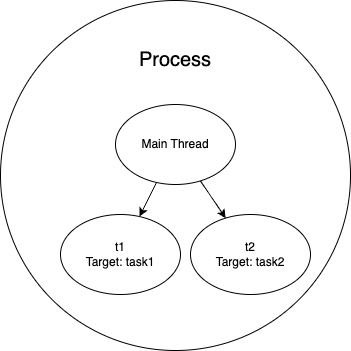
\includegraphics[width=0.5\textwidth]{/Users/khawaritzmi/Unhas/os_report_mid2024/a_class/asset/example.png}  % Sesuaikan nama file dan ukurannya
    \caption{Ini adalah gambar contoh dari multithreading.}
    \label{fig:contoh_gambar}
\end{figure}

Seperti yang terlihat pada Gambar \ref{fig:contoh_gambar}, inilah cara menambahkan gambar dengan keterangan.

\subsection{File Systems}
File systems provide a way for the operating system to store, retrieve, and manage data. This section explains:
\begin{itemize}
    \item File system structure
    \item File access methods
    \item Directory management
\end{itemize}

\subsection{Input and Output Management}
Input and output management is key for handling the interaction between the system and external devices. This section includes:
\begin{itemize}
    \item Device drivers
    \item I/O performance
\end{itemize}

\subsection{Deadlock Introduction and Prevention}
Explores the concept of deadlocks and methods for preventing them:
\begin{itemize}
    \item Deadlock conditions
    \item Deadlock prevention techniques
\end{itemize}

\subsection{User Interface Management}
This section discusses the role of the operating system in managing the user interface. Topics covered include:
\begin{itemize}
    \item Graphical User Interface (GUI)
    \item Command-Line Interface (CLI)
    \item Interaction between the user and the operating system
\end{itemize}

\subsection{Virtualization in Operating Systems}
Virtualization allows multiple operating systems to run concurrently on a single physical machine. This section explores:
\begin{itemize}
    \item Concept of virtualization
    \item Hypervisors and their types
    \item Benefits of virtualization in modern computing
\end{itemize}

\section{Assignments and Practical Work}
\subsection{Assignment 1: Process Scheduling}
Students were tasked with implementing various process scheduling algorithms (e.g., FCFS, SJN, and RR) and comparing their performance under different conditions.
\subsubsection{Group 1}
\begin{python}
    class Process:
    def __init__(self, pid, arrival_time, burst_time):
        self.pid = pid
        self.arrival_time = arrival_time
        self.burst_time = burst_time
        self.completion_time = 0
        self.turnaround_time = 0
        self.waiting_time = 0
\end{python}

\begin{table}[htbp] % Optional: For floating position
    \centering
    \begin{tabular}{|c|c|c|} % Defines number of columns and alignment (c = center, l = left, r = right). '|' creates vertical lines.
    \hline
    Header 1 & Header 2 & Header 3 \\ % Column headers
    \hline
    Row 1, Column 1 & Row 1, Column 2 & Row 1, Column 3 \\ % First row of data
    \hline
    Row 2, Column 1 & Row 2, Column 2 & Row 2, Column 3 \\ % Second row of data
    \hline
    \end{tabular}
    \caption{Your table caption} % Optional: For adding a caption
    \label{tab:your_label} % Optional: For cross-referencing the table
\end{table}
\subsection{Assignment 2: Deadlock Handling}
In this assignment, students were asked to simulate different deadlock scenarios and explore various prevention methods.

\subsection{Assignment 3: Multithreading and Amdahl's Law}
\noindent Tugas ini melibatkan perancangan skenario multithreading untuk menyelesaikan masalah komputasi intensif. Mahasiswa kemudian menerapkan Hukum Amdahl untuk menghitung peningkatan kecepatan teoritis program seiring dengan bertambahnya jumlah thread.

\textbf{Pertanyaan:}
\noindent Implementasikan sebuah program multithreading untuk menghitung nilai pi menggunakan metode Monte Carlo. Gunakan jumlah thread yang bervariasi (1, 2, 4, 8, dan 16) dan hitung waktu eksekusi untuk setiap kasus. Kemudian, terapkan Hukum Amdahl untuk menghitung peningkatan kecepatan teoritis, dengan asumsi 95% dari program dapat diparalelkan. Bandingkan hasil aktual dengan hasil teoritis dan jelaskan perbedaan yang mungkin terjadi.

\textbf{Jawaban:}
\begin{python}
import random
import threading
import time
def perkiraan_pi(titik_per_thread):
dalam_lingkaran = 0
for _ in range(titik_per_thread):
x = random.uniform(-1, 1)
y = random.uniform(-1, 1)
if xx + yy <= 1:
dalam_lingkaran += 1
return dalam_lingkaran
def hitung_pi(jumlah_thread, total_titik):
titik_per_thread = total_titik // jumlah_thread
threads = []
hasil = [0] * jumlah_thread
Copyfor i in range(jumlah_thread):
    thread = threading.Thread(target=lambda: hasil.__setitem__(i, perkiraan_pi(titik_per_thread)))
    threads.append(thread)
    thread.start()

for thread in threads:
    thread.join()

total_dalam = sum(hasil)
perkiraan_pi = 4 * total_dalam / total_titik
return perkiraan_pi
def main():
total_titik = 1000000
jumlah_thread_list = [1, 2, 4, 8, 16]
Copyfor jumlah_thread in jumlah_thread_list:
    waktu_mulai = time.time()
    hasil_pi = hitung_pi(jumlah_thread, total_titik)
    waktu_selesai = time.time()
    
    waktu_eksekusi = waktu_selesai - waktu_mulai
    print(f"Thread: {jumlah_thread}, Perkiraan Pi: {hasil_pi:.6f}, Waktu: {waktu_eksekusi:.4f} detik")
if name == "main":
main()

Penerapan Hukum Amdahl
def percepatan_amdahl(p, n):
return 1 / ((1 - p) + (p / n))
p = 0.95  # Asumsi 95% program dapat diparalelkan
jumlah_thread_list = [1, 2, 4, 8, 16]
print("\nPercepatan Teoritis (Hukum Amdahl):")
for n in jumlah_thread_list:
percepatan = percepatan_amdahl(p, n)
print(f"Thread: {n}, Percepatan: {percepatan:.2f}")
\end{python}


\subsection{Assignment 4: Simple Command-Line Interface (CLI) for User Interface Management}
Students were tasked with creating a simple **CLI** for user interface management. The CLI should support basic commands such as file manipulation (creating, listing, and deleting files), process management, and system status reporting.

\subsection{Assignment 5: File System Access}
In this assignment, students implemented file system access routines, including:
\begin{itemize}
    \item File creation and deletion
    \item Reading from and writing to files
    \item Navigating directories and managing file permissions
\end{itemize}

\section{Conclusion}
The  half of the course introduced core operating system concepts, including process management, scheduling, multithreading, and file system access. These topics provided a foundation for more advanced topics to be covered in the second half of the course.

\end{document}